\documentclass[12pt]{article}
\usepackage[a4paper, margin=2cm]{geometry}
\usepackage[english]{babel} % To obtain English text with the blindtext package
\usepackage{blindtext}
\usepackage{graphicx} % Required for inserting images
\usepackage{array, multirow} % For extra column formatting
\usepackage{amsmath, amssymb, cancel} %for equation environment
\usepackage{float}
\usepackage{parskip} % For gaps between para
\usepackage{setspace}
\usepackage{pdfpages}
\usepackage{abstract}
\usepackage[export]{adjustbox}
\usepackage{emptypage}
\usepackage{tocloft}
\usepackage[nottoc]{tocbibind}
\usepackage{hyperref, url}
\usepackage[table]{xcolor}
\usepackage{minted}
    \usemintedstyle{monokai}
\usepackage{caption,subcaption}
    \captionsetup{font=footnotesize,labelfont=bf}
\usepackage{tcolorbox}
    \newtcolorbox{mintedbox}{
        colback=backcolour,
        boxrule=0pt,
        sharp corners,
        width=\linewidth,
        left=0pt, right=0pt,
        top=3pt, bottom=3pt
    }
\usepackage[numbers]{natbib}

\cftsetindents{section}{0em}{2em}
\cftsetindents{subsection}{0em}{2em}

\renewcommand\cfttoctitlefont{\hfill\Large\bfseries}
\renewcommand\cftaftertoctitle{\hfill\mbox{}}

\graphicspath{ {./images/} }

\definecolor{blurple}{HTML}{5865F2}
\definecolor{backcolour}{HTML}{272823}

\hypersetup{
    colorlinks=true,
    linkcolor=black,
    urlcolor=black,
    citecolor=blurple,
}

\urlstyle{same}

\renewcommand{\arraystretch}{1.3}

\setcounter{secnumdepth}{5}
\setcounter{tocdepth}{5}
\newcommand\simpleparagraph[1]{%
  \stepcounter{paragraph}\paragraph*{\theparagraph\quad{}#1}}

\pagenumbering{arabic}

\hbadness=10001

%%%%%%%%%%%%%%%%%%%%%%%%%%%%%%%%%%%


\title{PHYC20040 Exp.4 Asteroids}
\author{Joana Adao}
\date{\today}

\begin{document}

\begin{titlepage}
    \begin{center}

        \begin{figure}[ht]
            
\includegraphics[width=\textwidth]{UCDLogo.png}
        \end{figure}
        
        \begin{figure}
            \centerline{
\includegraphics[width=\paperwidth]{UCDBanner.png}}
        \end{figure}

        \vspace{4cm}

        {\LARGE \bfseries PHYC20040 Exploring the Solar System}\\
        \vspace{0.75cm}
        {\Large Experiment No.4 Astrometry of Asteroids}
        
        \vspace{1cm}
    
    {\Large \textbf{26 March 2025}}

    \vspace{2cm}
    
    {\large \textbf{by Joana C.C. Adao (Student No. 23311051)}}\\

    \end{center}

   \clearpage

\end{titlepage}

\tableofcontents
\thispagestyle{empty}

\newpage

\begin{abstract}
\addtocontents{toc}{\protect\contentsline{section}{\textbf{Abstract}}{\hfill}{}}
\thispagestyle{empty}

The aim of this experiment was to utilise the astrometric parameter of parallax to measure the distance and angular velocity to the asteroid 1992 JB, consequently finding its tangential velocity component.
With the method of blinking, it was found that the asteroid appeared to move in a straight line North, and proper measurements done by the program with reference to catalogued stars (HST-GSC) backed this observation.
Through calculations, the distance to the asteroid from the Earth was found to be \textbf{43 157 822 km}, and the angular velocity of the asteroid was found to be \textbf{0.0126 "}. These values were then used to find the tangential component of the asteroid's
velocity, \textbf{2.64 km s}$\mathbf{^{-1}}$.
 
\end{abstract}
\newpage

%%%%%%%%%%%%%%%%%%%%%%%%%%%%%%%%%%%

\setcounter{page}{1}
\section{Theory} \label{sec:1}

\subsection{Introduction to Astrometry}

Astrometry is a type of astronomical measurement technique that focuses specifically on measuring the location of moving celestial objects within the sky plane \cite{ENDL2007887}.
This was one of the first techniques developed for searching planets around other stars, and remains a fundamental tool to astronomers to this day \cite{UCDastrometry,ENDL2007887}.

There are, of course, standard errors that come from measuring the movement of celestial objects through astrometric observations. This applies to both one's personal measurements and those found in star catalogues.
There will always be noise error when collecting photons from the targets, whether that be from background noise or from the target itself, photon distribution will vary between measurements at each different exposure time \cite{owen2000error}.
When measuring the position of an asteroid there will be tracking errors due to the fact that astroids move, sometimes producing trails that are neither straight nor uniformly illuminated, hence determining the centre is difficult \cite{owen2000error}.
These are examples of random errors that can be encountered, but there also exist systematic errors. The reference star catalogue may have possible zone errors, meaning stars have a bias for a particular region
of the sky that apply to any other asteroid measured in that sky region. The Hipparcos mission (1989-1993) was able to better pinpoint star's motion and position, thus effectively lessening this error \cite{owen2000error} and is being further
refined by the Gaia mission (2013-2025) \cite{hipparcos,gaiaesa}.

\subsection{Equatorial Coordinates}

\begin{figure}[hb]
    \centering
    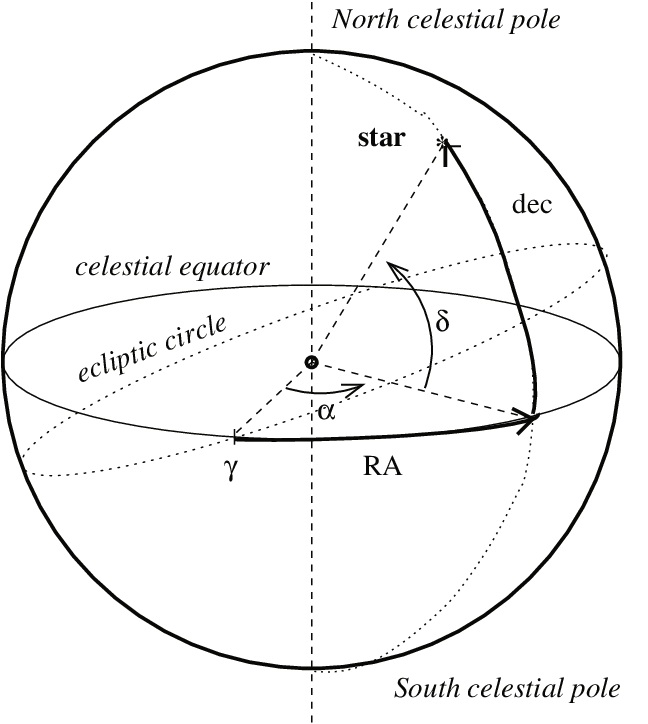
\includegraphics[width=.5\textwidth]{equatorial coords.png}
    \caption{Definition of equatorial coordinates system on the sky. Observer is at the centre of the sphere, which has an arbitrary radius of $\infty$ \protect\cite{equatorialcoords}.}
    \label{fig:1}
\end{figure}

The Equatorial coordinate system is the preferred system to pinpoint objects on the celestial spehere, part of the Celestial coordinate system. It is preferred to other celestial coordinate systems because equatorial coordinates are independent of the observer's location \cite{eqcoord1}.
This coordinate system is cosindered to be a celestial sphere of infinite radius with Earth at its centre, the Earth's poles coincident to the celestial poles (see Figure \ref{fig:1}) \cite{doody2001basics}.

The ecliptic plane represents the plane of Earth's orbit around the Sun, tilted 23.4$^{\circ}$ relative to the celestial equator \cite{doody2001basics}.

\subsubsection{Right Ascension and Declination}

The right ascension (RA) and declination (Dec) are the equatioral equivalent of longitude and latitude respectively \cite{eqcoord1,doody2001basics}.

\textbf{Right Ascension (RA)} is expressed in hours (h), minutes (m), and seconds (s) \cite{doody2001basics}. The sky would appear to turn the full 360$^{\circ}$ in 24 hours, so an hour of RA would be 15$^{\circ}$ \cite{doody2001basics}. RA starts being measured at the vernal equinox ($\gamma$ in Figure \ref{fig:1}),
which is the point where the celestial equator intersects the ecliptic \cite{eqcoord1}.

\textbf{Declination (Dec)} is expressed in degrees ($^{\circ}$), minutes ('), and seconds (") \cite{doody2001basics}. At the celestial equator, declination is 0$^{\circ}$, the North Pole is +90$^{\circ}$, and the South Pole would then be -90$^{\circ}$ \cite{doody2001basics}.

\subsubsection{Reference Star Catalogues}

\textbf{FK5}, the Fifth Fundamental Catalogue, is a star catalogue containing 1535 classical fundamental stars and the successor to the FK4 system \cite{warren1990fifth}. It was publised in 1988, with an extension to the catalogue being published in 1991, adding 3117 new stars \cite{lattanzi1993fk5}. These catalogues served as a foundation to the International
Celestial Referency System (ICRS) and then were consequently superseded by Hipparcos \cite{wielensixth}. 

\textbf{Guide Star Catalogue (GSC)} was primarily to provide guide star information for the Hubble Space Telescope (HST) for observational planning support, but has since been expanded to provide similar support to other telescopes, such as the James Webb Space Telescope (JWST) and GAIA \cite{lasker2008second}.
The GSC2.3 has catalogued 945 592 683 (945 million) objects through astrometry and photometry classifications \cite{lasker2008second}, while the first version (GSC-I) had only 19 million bright objects (magnitude greater than 16) \cite{hstgsc}. The GSC-II catalogues extend to fainter magnitudes, offering better positional accuracy.

\subsection{Stellar Parallax} \label{sec:1.3}

Parallax is one of the key parameters to astrometric observations \cite{luri2018gaia}.
Stellar parallax is the apparents movement of a star against the background of more distant stars as the Earth orbits the Sun (see Figure \ref{fig:2}) \cite{esaparallax,lcoparallax,britparallax}. 
The relationship between the bright object's distance and the angle of parallax is given by \cite{lcoparallax},

\vspace{-2ex}
\begin{gather*}
    d = \frac{\dfrac{B}{2}}{tan\left(\dfrac{\Theta}{2}\right)}
\end{gather*}

Where d is the distance, B is the baseline, and $\Theta$ is the parallax angle.
Measurements of parallax are hard to get accurate to less than 0.01 arsec due to the atmosphere of the Earth \cite{lcoparallax}, but missions like Hipparcos and the Tycho Catalogue were able to refine this further, with Hipparcos to accuracy of 1 milliarsec \cite{perryman1997hipparcos}
and the Tycho Catalogue at precisions of 7-25 milliarsec, dependent of magnitudes \cite{hog1997tycho}.

\begin{figure}[H]
    \centering
    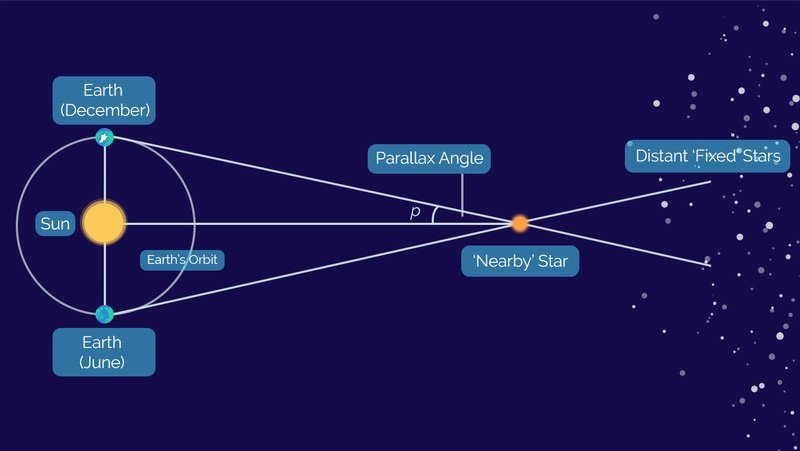
\includegraphics[width=.75\textwidth]{parallax.jpg}
    \caption{Diagram of stellar parallax, showing how the 'nearby' stars appear to move against the 'fixed' stars when Earth is at different positions in its orbit around the Sun \protect\cite{lcoparallax}.}
    \label{fig:2}
\end{figure}

\subsection{Asteroids}

Asteroids, sometimes called minor planets \cite{nasaasteroid}, are small rocky planetary bodies \cite{asphaug2009growth} that don't quite meet the requirements to be classified as a planet due to their size and irregular shape \cite{hubbleasteroid}.
Many come about as debris left behind by failed-planet objects or from collisions \cite{hubbleasteroid,nasaasteroid,asphaug2009growth}. Many of early asteroids even grew large enough to undergo thermal differentiation, leading to scattered fragments of their metal0rich cores and, less
frequently, their mantles and crusts \cite{asphaug2009growth}. Asteroids differ from comets in this way, as comets comprise of dust and ice rather than being rocky \cite{hubbleasteroid}.
Most asteroids in the Solar System orbit the Sun between Mars and Jupiter, it being the main asteroid belt (see Figure \ref{fig:3}) \cite{nasaasteroid}.

\begin{figure}[H]
    \centering
    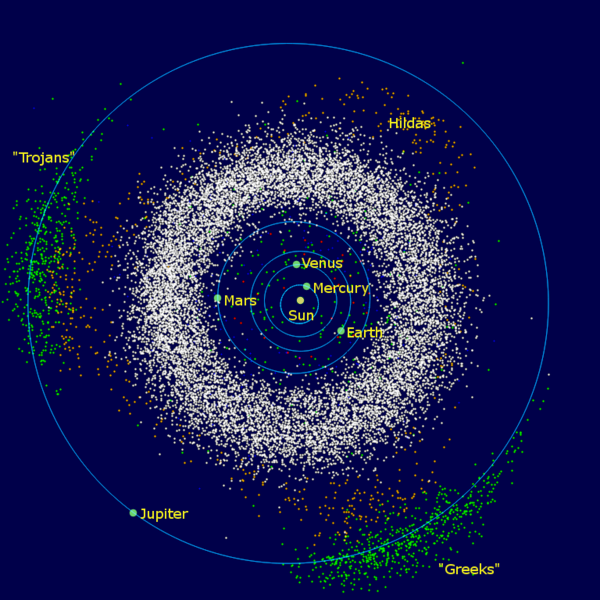
\includegraphics[width=.5\textwidth]{asteroids solar system.png}
    \caption{The asteroids of the inner Solar System and Jupiter: the belt is located between the orbits of Jupiter and Mars \protect\cite{wikiasteroidbelt}.}
    \label{fig:3}
\end{figure}

\newpage

\section{Methodology} \label{sec:2}

The Contemporary Laboratory Experiences in Astronomy (CLEA) software is used for this exercise. The program 'Astrometry of Asteroids' is made use of for the following measurements.

\subsection{Part I: Finding Asteroids by Blinking Images}

For this section, the "blinking" method is made use of to compare between two images, taken at different times, observing the same region of the sky. Once two reference stars, usually quite bright and at opposite side of the image diagonal to one another for maximum accuracy, the 
two images are switched at defined intervals of a few seconds. By continuously switching between the two images any movement between them can be observed, which can be indicative of an asteroid. A hand-drawn image or computer-rendered representation of the trajectory of the asteroid can be deciphered by blinking multiple images,
all taken at different times. For this exercise, the asteroid 9058 (1992 JB) was observed.

\subsection{Part II: Measuring the Equatorial Coordinates of an Asteroid by Comparing It to Positions of Known Stars in the HST-GSC}

The CLEA 'Astrometry of Asteroids' program includes a "measure" feature that compares the position of known stars in the GSC catalogue to the stars in the pictures taken of the sky region where the 1992 JB asteroid can be found. To find the locatoin of the asteroid in equatorial coordinates, its
location is triangulated with (at least) 3 other known stars. These are marked on the GSC catalogue window first before being located in the iamge of the sky region. After locating the object (asteroid) position, the computer software does the calculations to provide a list of information, including the desired
RA and Dec measurements. The results can be tabulated for reference.

\subsection{Part III: Angular Velocity of Asteroid 1992 JB}

This section of the experiment focuses on calculating the angular velocity of the astroid 1992 JB using the information gathered in Part II. After converting both the RA and Dec findings to seconds, the Pythagorean theorem can be
redefined to suit current purposes:

\vspace{-2ex}
\begin{gather} \label{eq:1}
    c = \sqrt{a^2 + b^2} \quad \implies \quad \Delta \theta = \sqrt{(\Delta \text{RA(")})^2 + (\Delta \text{Dec(")})^2}
\end{gather}

where $\Delta$Dec(") is the difference in declination measurements and $\Delta$RA(") can be calculated with:

\vspace{-2ex}
\begin{gather} \label{eq:2}
    \Delta \text{RA(")} = \Delta \text{RA(sec)} \times 15 \times cos(\text{Dec}(^{\circ}))
\end{gather}

and $\Delta$RA(sec) is the difference in right ascension measurements. This value can then be used to find the angular velocity,

\vspace{-2ex}
\begin{gather} \label{eq:3}
    \mu = \frac{\Delta \theta}{\Delta t}
\end{gather}

where $\Delta$t is the difference in time between both images that are being compared in seconds.

\subsection{Part IV: Measuring the Distance of Asteroid 1992 JB by Parallax}

For this section of the experiment the concept of measuring distance through parallax as discussed in §\ref{sec:1.3} is revisited. Two images of the same region of the sky are compared simultaneously, one taken at a Western location (Flagstaff, Arizona) and another taken at an
Eastern loaction (Hamilton, New York). The distance between these two telescopes, 3172 km, is taken as the baseline. The distance to the asteroid can then be calculated using

\vspace{-2ex}
\begin{gather} \label{eq:4}
    D = 206 \; 265 \frac{B}{\Delta \theta}
\end{gather}

where D is the distance to the asteroid, B is the baseline (3172 km), $\Delta \theta$ is the parallax angle and can be calculated using the same formula as Eq. \ref{eq:1}, and 206 265 is the arcsec equivalent of 1 radian.

The same process to calculate $\Delta \theta$ as was used in Part III is used again and then substituted in to the equation to find the distance to the asteroid in kilometres.

\subsection{Part V: The Tangential Velocity of Asteroid 1992 JB}

This is a continuation of Part III and Part IV, using the angular velocity ($\mu$) and the distance (D) found in both to then calculte the tangential velocity using the following formula,

\vspace{-2ex}
\begin{gather} \label{eq:5}
    V_t = \frac{\mu \times D}{206 \; 265}
\end{gather}

where $V_t$ is the tangential velocity in kilometres per second, $\mu$ is the angular velocity calculated in Part III, D is the distance to the asteroid calculated in Part IV, and 206 265 is the arcsec equivalent of 1 radian.

\newpage

\section{Results and Discussion} \label{sec:3}

\subsection{Part I: 1992 JB Path Through Blinking}

The freehand sketch of the region of the sky being observed containing the asteroid 1992 JB is given in Figure \ref{fig:4} below. Each location placement was visually estimated through blinking, any error in positioning is purely human error.

\begin{figure}[H]
    \centering
    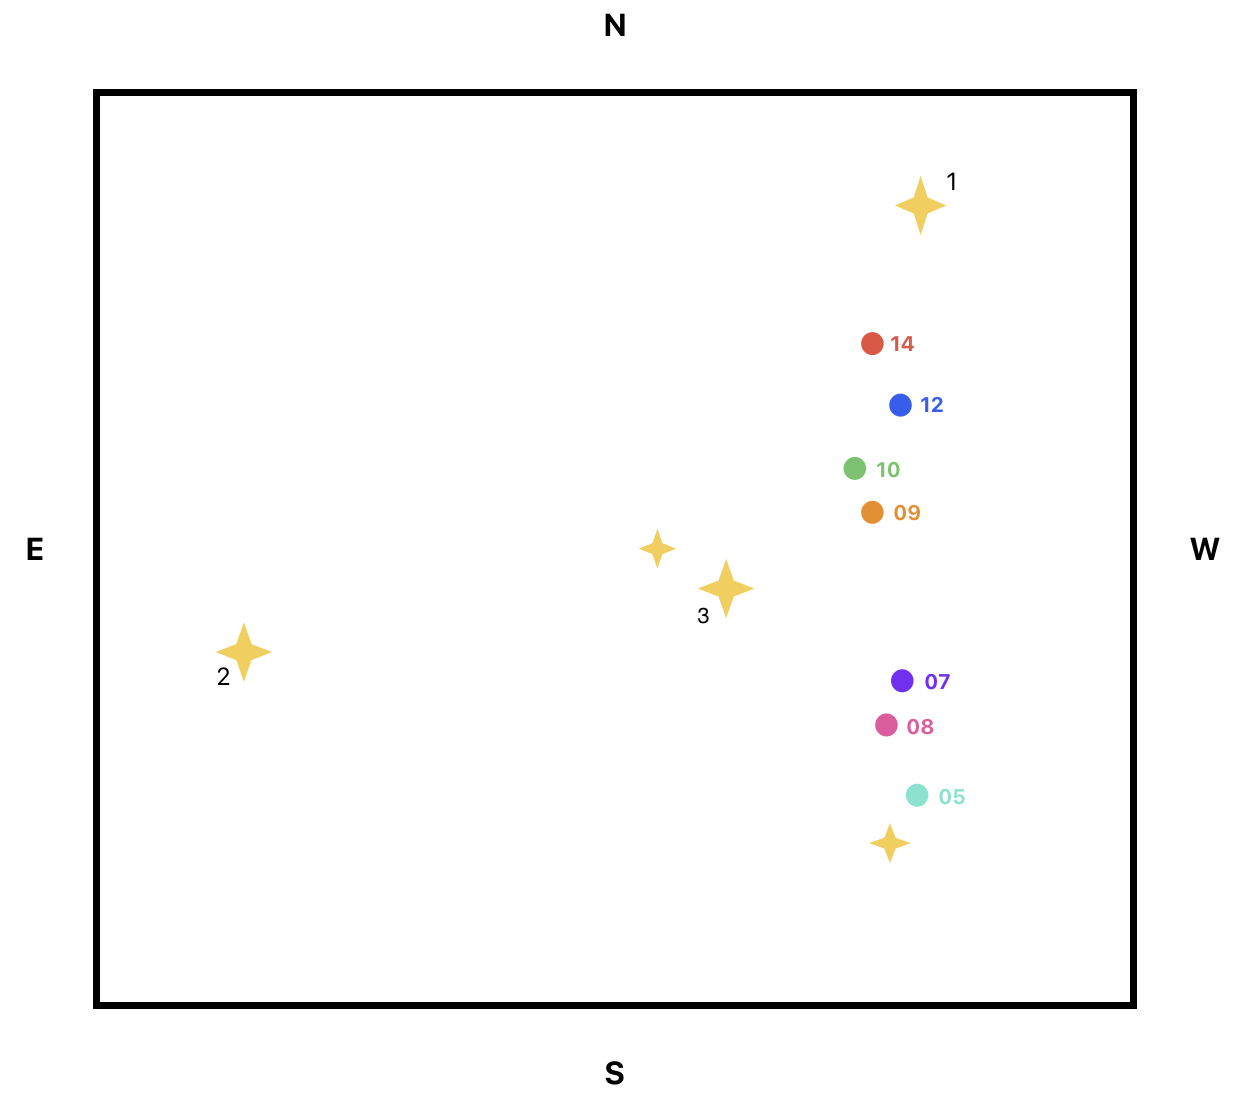
\includegraphics[width=.8\textwidth]{freehand asteroid.png}
    \caption{Freehand sketch of the asteroid path through the blinking of images of the 1992 JB asteroid. \newline \textit{Number markings of the asteroid correspond to image file names, e.g. 92JB05.fts is the "05" asteroid.}}
    \label{fig:4}
\end{figure}

As can be observed, the asteroid follows a straight line North, which is what is to be suspected.

\subsection{Part II: 1992 JB in Equatorial Coordinates}

The chosen reference stars can be seen labelled "1", "2", and "3" in Figure \ref{fig:4}. Compared to the HST-GSC povided by the CLEA software, the coordinates for these stars are given in Table \ref{tab:1}

\begin{table}[H]
    \centering
    \caption{Table of the reference star equatorial coordinates.}
    \label{tab:1}
    \resizebox{.7\textwidth}{!}{%
        \begin{tabular}{
        >{\columncolor[HTML]{EFEFEF}}c ccc}
        \textbf{Reference Star} & \textbf{ID \#} & \textbf{RA (h  m  s)} & \textbf{Dec ($^{\circ}$  '  ")} \\ \hline
        \#1 & 00936-00017 & 15  30  36.23 & 11  16  20.8 \\
        \#2  & 00936-00007 & 15  30  46.56 & 11  15  00.8 \\
        \#3  & 00936-00754 & 15  30  39.39 & 11  15  14.2
        \end{tabular}%
    }
\end{table}

The equatorial coordinates measured by the CLEA program for the 1992 JB asteroid are then tabulated for readability, shown in Table \ref{tab:2}.

\begin{table}[H]
    \centering
    \caption{Table of the measured RA and Dec coordinates for each image of the 1992 JB asteroid}
    \label{tab:2}
    \resizebox{.75\textwidth}{!}{%
        \begin{tabular}{
        >{\columncolor[HTML]{EFEFEF}}c ccc}
        \textbf{File Name} & \textbf{Time (UT) (h  m  s)} & \textbf{RA (h  m  s)} & \textbf{Dec ($^{\circ}$  '  ")} \\ \hline
        92JB05 & 04  53  00 & 15  30  38.70 & 11  14  06.2 \\
        92JB07 & 05  03  00 & 15  30  38.70 & 11  14  14.6 \\
        92JB08 & 05  09  00 & 15  30  38.72 & 11  14  18.4 \\
        92JB09 & 06  37  30 & 15  30  38.70 & 11  15  26.8 \\
        92JB10 & 06  49  00 & 15  30  38.70 & 11  15  34.6 \\
        92JB12 & 06  57  00 & 15  30  18.69 & 11  15  41.2 \\
        92JB14 & 07  16  00 & 15  30  18.68 & 11  15  54.7
        \end{tabular}%
    }
\end{table}

As the asteroid appears to be moving in a straight line up, it was expected for the RA values to be approximately the same, which is what is numerically observed.

\subsection{Part III: The Angular Velocity of 1992 JB}

According to the findings shown in Table \ref{tab:2}, the time between 92JB05 and 92JB14 (column 2) is found in seconds:

\vspace{-2ex}
\begin{align*}
    \text{\textbf{92JB14}} : 7 \: \text{h} \:\: 16 \: \text{m} \quad \rightarrow \quad 26 \; 160 \: \text{s} \\
    \text{\textbf{92JB05}} : 4 \: \text{h} \:\: 53 \: \text{m} \quad \rightarrow \quad 17 \; 580 \: \text{s}
\end{align*}

The difference in time, $\Delta$t, is then found to be \textbf{8580 s}. The declination for 92JB05 and 92JB14 (column 4) is also found in seconds:

\vspace{-2ex}
\begin{align*}
    \text{\textbf{92JB14}} : 11 \: ^{\circ} \:\: 15 \: \text{'} \:\: 54.7 \: \text{"} \quad \rightarrow \quad 40 \; 554.7 \: \text{"} \\
    \text{\textbf{92JB05}} : 11 \: ^{\circ} \:\: 14 \: \text{'} \:\: 06.2 \: \text{"} \quad \rightarrow \quad 40 \; 446.2 \: \text{"}
\end{align*}

The difference in declination, $\Delta$Dec(") is then found to be \textbf{108.5 "}. To get this value in degrees for the $\Delta$RA(") calculations, divide the seconds value by 3600 to get \textbf{0.03} $^{\circ}$.
The right ascension for 92JB05 and 92JB14 (column 3) is now found in seconds:

\vspace{-2ex}
\begin{align*}
    \text{\textbf{92JB14}} : 15 \: \text{h} \:\: 30 \: \text{m} \:\: 38.68 \: \text{s} \quad \rightarrow \quad 58 \; 838.68 \: \text{s} \\
    \text{\textbf{92JB05}} : 15 \: \text{h} \:\: 30 \: \text{m} \:\: 38.70 \: \text{s} \quad \rightarrow \quad 58 \; 838.70 \: \text{s}
\end{align*}

The difference in right ascension, $\Delta$RA(s) is then found to be \textbf{0.02 s}. Using Eq. \ref{eq:2}, $\Delta$RA(") is calculated:

\vspace{-2ex}
\begin{gather*}
    \Delta \textbf{RA} (") = (0.02) \times (15) \times \cos (0.03) = \mathbf{0.29} \: "
\end{gather*}

So the $\Delta$RA(") is found to be \textbf{0.29 "}. With both $\Delta$RA and $\Delta$Dec now in seconds ("), Eq. \ref{eq:1} can be used to find $\Delta \theta$:

\vspace{-2ex}
\begin{gather*}
    \Delta \theta = \sqrt{(0.29)^2 + (108.5)^2} = \mathbf{108.5} \: "
\end{gather*}

With $\Delta \theta$ and $\Delta$t now found Eq. \ref{eq:3} can be used to find the angular velocity of 1992 JB asteroid:

\vspace{-2ex}
\begin{gather*}
    \mu = \frac{108.5}{8580} = \mathbf{0.0126} \: \text{\textbf{"/second}} 
\end{gather*}

Therefore, the angular velocity of the 1992 JB asteroid on the 23rd of May, 1992 is calculated to be \textbf{0.0126 seconds}.

\subsection{Part IV: 1992 JB Distance by Parallax}

The angle of the photos as taken from Flagstaff, Arizona and Hamilton, New York appear to be different due to parallax, as discussed in §\ref{sec:1.3}. The distance between the two observatories is \textbf{3172 km}, this will be taken as the baseline (B) for Eq. \ref{eq:4}.
The table for the measurements of the 1992 JB asteroid as taken from the ATEAST and ATWEST locations is tabulated in Table \ref{tab:3} below.

\begin{table}[H]
    \centering
    \caption{Table of coordinate measurements for 1992 JB asteroid for ATEAST and ATWEST.}
    \label{tab:3}
    \resizebox{.45\textwidth}{!}{%
        \begin{tabular}{
        >{\columncolor[HTML]{EFEFEF}}c cc}
        \textbf{File} & \textbf{RA (h  m  s)} & \textbf{Dec ($^{\circ}$  '  ")} \\ \hline
        ATEAST        & 15  30  37.72         & 11  15  36.1                    \\
        ATWEST        & 15  30  38.69         & 11  15  41.2                   
        \end{tabular}%
    }
\end{table}

These coordinates are both converted into seconds as before for ease of calculations, tabulated for readability in Table \ref{tab:4} below.

\begin{table}[H]
    \centering
    \caption{Table of coordinate measurements for 1992 JB asteroid for ATEAST and ATWEST.}
    \label{tab:4}
    \resizebox{.45\textwidth}{!}{%
    \begin{tabular}{
        >{\columncolor[HTML]{EFEFEF}}c cc}
        \textbf{File} & \textbf{RA (h  m  s)} & \textbf{Dec ($^{\circ}$  '  ")} \\ \hline
        ATEAST        & 15  30  37.72         & 11  15  36.1                    \\
        ATWEST        & 15  30  38.69         & 11  15  41.2                   
        \end{tabular}%
    }
\end{table}

The difference in declination, $\Delta$Dec(") is then found to be \textbf{5.1 "} and $\Delta$RA(s) to be \textbf{0.97 s}. This value is once again converted into degrees for calculating $\Delta$RA(") by multiplying by 3600 to get \textbf{0.00142} $^{\circ}$. 
The right ascension $\Delta$RA(") is found to be, using Eq. \ref{eq:2}:

\vspace{-2ex}
\begin{gather*}
    \Delta \textbf{RA} (") = (0.97) \times (15) \times \cos (0.00142) = \mathbf{14.28} \: "
\end{gather*}

So $\Delta$RA(") is then found to be \textbf{14.28 "}. This value and the one found for $\Delta$Dec(") can be used in Eq. \ref{eq:1} to find the angle of parallax ($\Delta \theta$):

\vspace{-2ex}
\begin{gather*}
    \Delta \theta = \sqrt{(14.28)^2 + (0.00142)^2} = \mathbf{15.16} \: "
\end{gather*}

Therefore the angle of parallax $\Delta \theta$ is found to be \textbf{15.16 "}. To find the distance to asteroid 1992 JB, Eq. \ref{eq:4} is used,

\vspace{-2ex}
\begin{gather*}
    D = 206 \; 265 \; \frac{3172}{15.16} = \mathbf{43 \; 157 \; 822} \text{\textbf{km}}
\end{gather*}

So the distance to asteroid 1992 JB on the 23rd of May, 1992 is found to be \textbf{43 157 822 km}. In astronomical units, this would be \textbf{0.288 AU} (from Earth). This is not the closest this asteroid can get to Earth as, at perihelion, its distance from the sun is 1.00 AU.
In fact, on the 21st of April, 2025 the asteroid 1992 JB will be 15 291 069 km from Earth. Its proximity to Earth means that this asteroid is classed as a near-Earth asteroid (NEA) \cite{1992jb}. 
Compared to the distance of Earth to the moon, which 0.0025 AU, the 1992 JB asteroid was 115.2 times further away from the Earth on the 23rd of May, 1992. At its closest point, 1992 JB is 0.08 AU from Earth. Despite its proximity to Earth, orbital simulations have not considered this asteroid as hazardous \cite{1992jb}. 

\subsection{Part V: 1992 JB Tangential Velocity}

Using Eq. \ref{eq:5} and the values found for the angular velocity $\mu$ in Part III and distance D in Part IV, the tangential velocity of the 1992 JB asteroid can be found:

\vspace{-2ex}
\begin{gather*}
    V_t = \frac{0.0126 \times 43 \; 157 \; 822}{206 \; 265} = \mathbf{2.64} \: \text{\textbf{km s}}\mathbf{^{-1}}
\end{gather*}

So the tangential component to the velocity of the 1992 JB asteroid $V_t$ is found to be \textbf{2.64 km s}$\mathbf{^{-1}}$.

\newpage

\section{Conclusion} \label{sec:4}

This experiment was successful in demonstrating how to use parallax to find the distance to distant celestial objects, in this case the asteroid 1992 JB. Through the method of blinking in Part I, the asteroid was first observed to be moving in a straight line North, and this observation
was confirmed in Part II when the equatorial coordinates of the asteroid at different times was found and the right ascension coordinates (RA) remained approximately the same.

By comparing the difference in coordinates and time of the earliest (92JB05) and latest (92JB14) images of the asteroid in Part III the angular velocity of the 1992 JB asteroid was found to be \textbf{0.0126 "} on the 23rd of May, 1992.

A similar process was followed in Part IV by comparing the coordinates of the 1992 JB asteroid at different locations, one East (Flagstaff, Arizona) and one West (Hamilton, New York), to find the angle of parallax of the observation of the asteroid. This measurement was then used, in tandem with the distance between
both participating observatories, to calculate the distance to the asteroid from Earth, \textbf{43 157 822 km} on the 23rd of May, 1992. In astronomical units this would be 0.288 AU, but by consulting a catalogue of asteroids it was found that the closest the 1992 JB asteroid can get to Earth is 0.08 AU \cite{1992jb}.
This would mean that the 1992 JB asteroid is classified as a near-Earth asteroid (NEA).

With the values calculated for both angular velocity in Part III and distance in Part IV, the tangential component of velocity of the 1992 JB asteroid was found to be \textbf{2.64 km s}$\mathbf{^{-1}}$. By, once again, consulting a catalogue of asteroids it is found that the average orbital velocity of the 1992 JB asteroid is 
23.89 km s$^{-1}$. The extreme difference in values likely arises due to the fact that the orbital velocity value is made up of both the radial and tagential components and only the tangential component was found. As the 1992 JB asteroid was classified as a near-Earth asteroid, one would assume that the orbital velocity of the asteroid 
would be similar to that of Earth's and, according to calculations done in this experiment, this would appear to not hold, once again most probably due to only the tangential component being calculated. For total accuracy in the comparison of values to waht would be expected, the calcualtions from the experiment should be 
expanded further to calculate the orbital velocity of the asteroid rather than just a singular component.

\newpage

%%%%%%%%%%%%%%%%%%%%%%%%%%%%%%%%%%%

\bibliographystyle{IEEEtran}
\bibliography{References} \label{sec:ref}

\vspace{1.5cm}

\listoffigures

\listoftables

\newpage

\section*{Appendix: Questions}
\addcontentsline{toc}{section}{Appendix: Questions}

\textbf{Q1. There are two perpendicular components to the velocity of the asteroid. One is the tangential component calculated above. What is the second component? Draw the velocity vectors and label both components.}\\

The other velocity component is the radial velocity component, shown below.

\begin{figure}[H]
    \centering
    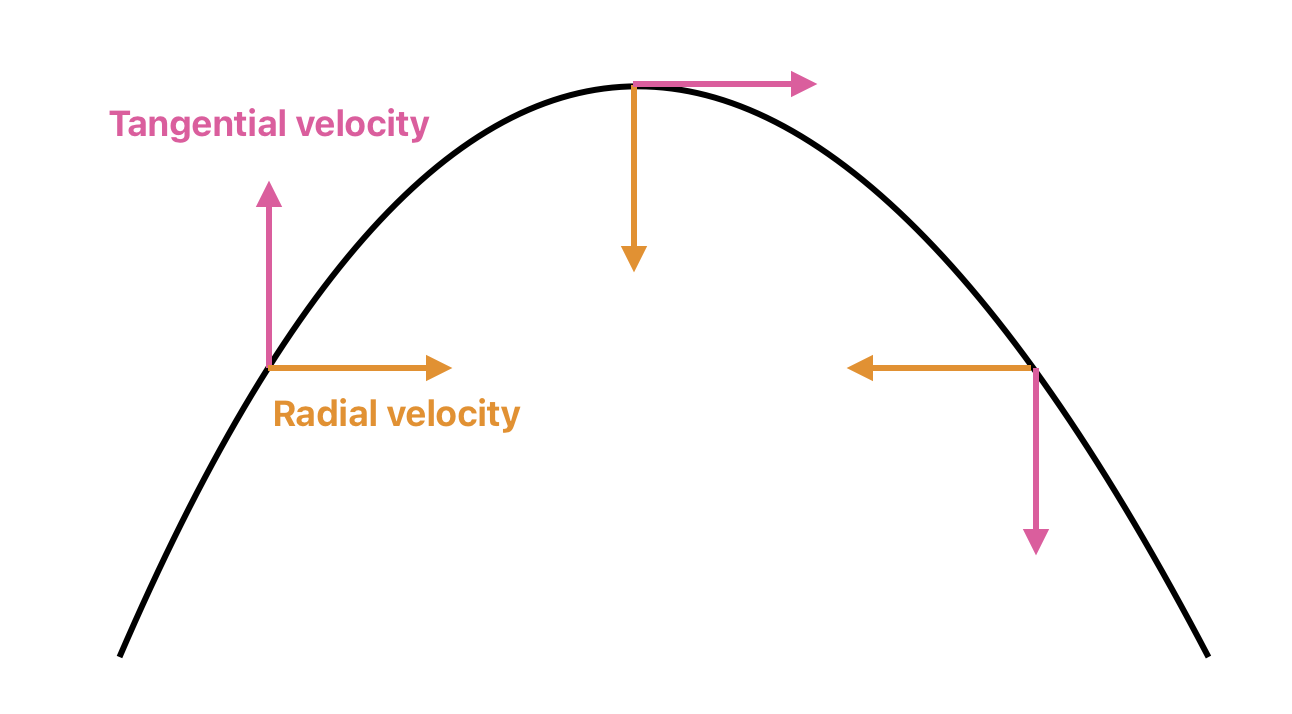
\includegraphics[width=.5\textwidth]{vel comp.png}
    \caption*{Sketc of the tangential and radial velocity components on a curve.}
\end{figure}

\textbf{Q2. What is the orbital radius of Earth? What is another name for this distance? Express this distance in both AU and km. Draw a picture of the Earth orbiting the Sun to help you answer this question.}\\

The distance from the Earth to the Sun, Earth's orbital radius, is 1.00 AU as per definition. In kilometres, this is 1.496 $\times 10^8$ km. Earth's orbit around the Sun is sketched below.

\begin{figure}[H]
    \centering
    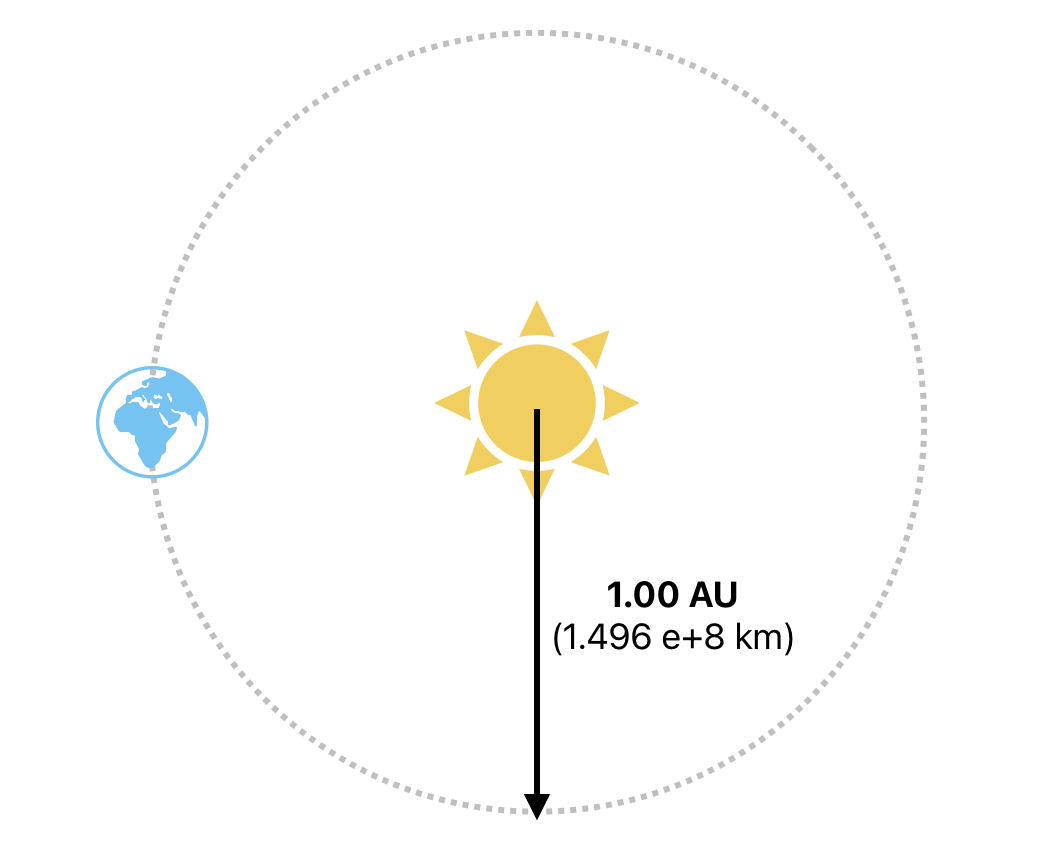
\includegraphics[width=.5\textwidth]{sunearth orbit.png}
    \caption*{The Earth's orbital distance around the Sun sketch (not to scale).}
\end{figure}

\textbf{Q3. What is the orbital period of the Earth? Express this answer in both years and seconds.}\\

The orbital period of Earth is 1 year, or 31 558 118.4 seconds (as the orbital period, in days, is $\sim$356.256).

\textbf{Q4. Using the information from questions 2 and 3, we can calculate the orbital velocity of the Earth for comparison with the orbital velocity of the asteroid. Velocity can be calculated using this equation: velocity = distance / time.
Using the orbital radius of the Earth, divide the circumference of the Earth's orbit ($\mathbf{2 \pi R_{OE}}$) with its orbital period (T) is seconds to determine the Earth's orbital velocity.} \\

\begin{gather*}
    V_O = \frac{2 \pi R_{OE}}{T} = \frac{2 \pi (1.496 \times 10^{8})}{31 \; 558 \; 118.4} \simeq \mathbf{29.8} \: \textbf{km s} \mathbf{^{-1}}
\end{gather*}

\textbf{Q5. Would you expect an asteroid to have a lower or higher orbital velocity than the Earth? Why? Look at the orbital velocity of planets in our Solar System in an appendix in your text for a pattern on which to base your answer.}\\

An asteroid's orbital velocity depends on the orbital radius, so you would expect an asteroid closer to the Sun to have a higher orbital velocity than one located farther away. \\

\textbf{Q6. How does this asteroid's tangential component of velocity compare to the orbital velocity of the earth? Does it follow the pattern of orbital velocities of other objects in the Solar System?}\\

According to official databases, the average orbital velocity of the 1992 JB asteroid is 23.89 km s$^{-1}$ \cite{1992jb}, which aligns much better with what is expected (similar to Earth's orbital velocity at perihelion) than what was calculated (2.64 km s$^{-1}$). With a much smaller orbital velocity as was calculated, the orbit of the asteroid would be
assumed to be much larger.

\end{document}